\documentclass[..\EOYR.tex]{subfiles}

\begin{document}

%\section{The separation and path of the Gulf Stream}
\section{The Dynamics of the Gulf Stream}
\todo{Maybe retitile}

The Gulf stream separates at Cape Hatteras, skirts the Grand Banks at Newfoundland and then heads Eastwards towards western Europe. However, in many moderate resolution climate models this separation occurs further north than observed and turns more sharply to the East, as noted in \citep{Hurlburt2008} and often misses off the Grand Banks, heading straight towards Europe. This can lead to what modellers refer to as the "blue spot of death" \citep{Gnanadesikan2007}, a patch of colder than observed SSTs resulting from the lack of heat at Newfoundland normally brought up by the Gulf Stream.

The exact cause for the path of the Gulf Stream is unknown, though it has been a research topic for many years and is still a popular topic amongst researchers today. A recurring theme when looking into the separation of the Gulf Stream is the mention of bathymetry. It is thought \citep{Gula2014}\citep{NaveiraGarabato2013}\citep{Nikurashin2012a} that the ocean dynamics resulting from the interaction of the Gulf Stream and the deep western boundary current (DWBC) with the bathymetry in the North Atlantic could cause the turbulence required to direct the Gulf Stream along its path. A sudden change in the direction of the Gulf Stream just off the coast at South Carolina and Georgia has been attributed by \citep{Gula2014} to the Charleston Bump, a topographical feature which raises the ocean floor, from a depth of 600m on the surrounding Blake Plateua to 200m. Hence it is clear that bathymetry can strongly impact the direction of ocean currents.


\subsection{Subpolar Gyre \& subtropical gyre?}

\subsection{The Effects of topography}

\citep{NaveiraGarabato2013} \td{explain} the dynamics of the ocean as a balance between the wind stress causing acceleration on the surface against the deceleration of the pressure forces resulting from the bathymetry.
The extent of the impact of topography on ocean dynamics can be seen by examining the difference between flat bottom models and models with realistic bathymetry. \td{Introduce the equations here with bpt and jebar? one of the papers does a really good job of justifying this - maybe greatbatch or gula? include some of the Gula or Yeager figures}

There are many ways to look into these differences, but we will focus mainly on two terms, the bottom pressure torque and the Joint Effect of Baroclinicity And Relief (JEBAR), as used by \citep{Greatbatch1991}, \citep{Bell1999}, \citep{Gula2014} as well as many others. 


\subsubsection*{The Joint Effect of Baroclinicity and Relief (JEBAR)}

The JEBAR term was first introducted to account for the effects of topography and baroclinicity after \td{unrealistic results yielded from the more traditional flat-bottomed models of XXX and XXX}. \citep{Ezer2016b} states that this term is crucial for accurate Gulf Stream separation. \\
The term arises from the \td{potential/barotropic} vorticity equation after taking the curl of the vertically averaged zonal and meridional flow.
\par
We will follow the derivation of the JEBAR and bottom pressure torque terms used in \citep{Greatbatch1991} as it shows the \td{barotropic vorticity equation} as a combination of a JEBAR term and a wind term, demonstrating the balance referenced by \citep{NaveiraGarabato2013}\todo{maybe cite someone else? GV?}.

First we introduce the horizontal momentum equations \ref{EQN:momU} \& \ref{EQN:momV}, the hydrostatic relation \ref{EQN:Hydrostatic} and the continuity equation \ref{EQN:Continuity}\todo{continuity or mass conservation} determining flow in spherical coordinates

\input{equations/MomU.tex}
\begin{equation}
    fu=-\frac{1}{a\rho_0}\frac{\partial p}{\partial \phi} + \frac{1}{\rho_0}\frac{\partial\tau_{z\phi}}{\partial z}
\label{EQN:MomV}
\end{equation}

\begin{equation}
    0=-\frac{\partial p}{\partial z} - \rho_0 b
\label{EQN:Hydrostatic}
\end{equation}

\begin{equation}
    \frac{1}{a\cos\phi}\left(\frac{\partial u}{\partial\lambda} + \frac{\partial}{\partial\phi}\left(v\cos\phi\right)\right) + \frac{\partial w}{\partial z}=0
\label{EQN:Continuity}
\end{equation}


taking the coordinates with $\lambda$ as the longitude, $\phi$ as the latitude and $z$ as the altitude from the sea surface $\left(z=0\right)$ upwards.
The remaining terms are: $u$, $v$, and $w$ are the zonal, meridional and vertical velocity; $a$ is the Earth's radius; $\rho_0$ is the density of seawater; $p$ is the pressure perturbation; $b=g\frac{\left(\rho-\rho_r\right)}{\rho_0}$ is the negative buoyancy (where $\rho_r=\rho_r(z)$, the horizontally averaged denisty at depth $z$, and $g$ is the acceleration due to gravity); and $\tau_{z\lambda}$ and $\tau_{z\phi}$ are \td{turbulent Reynolds stresses}.\\
In line with the \citep{Greatbatch1991} derivation and \td{citep{Mellor TODO}} we neglect the local time derivative, nonlinear advection and horizontal Reynolds stress as we are focused on the vertical integration of the equations.\todo{See paper for explanation or not?}


First we introduce the notation
\begin{equation}
    U=\int_{-H}^0 u \, \text{d}z,\quad V=\int_{-H}^0 v \, \text{d}z.
\label{EQN:UVInt}
\end{equation}

We now establish a streamfunction $\psi$ satisfied by $U$ and $V$ by taking the vertical integral of \ref{EQN:Continuity}
\begin{equation}
    \frac{1}{a\cos\phi}\left(\frac{\partial U}{\partial\lambda} + \frac{\partial}{\partial\phi}\left(V\cos\phi\right)\right)=0.
\label{EQN:VIntContinuity}
\end{equation}

We then have the define the required streamfunction by
\begin{equation}
    aU=-\frac{\partial\psi}{\partial\phi}\,,\quad aV\cos\phi=\frac{\partial\psi}{\partial\lambda}.
\label{EQN:Streamfunction}
\end{equation}

%
Taking the vertical averages of \ref{EQN:MomU} and \ref{EQN:MomV} gives
\begin{equation}
    -\frac{fV}{H} = -\frac{1}{Ha\rho_0\cos\phi}\int_{-H}^0\frac{\partial p}{\partial\lambda} \, \text{d}z + \frac{1}{H\rho_0}\left[\tau_\lambda^s-\tau_\lambda^b\right]
\label{EQN:VAvU}
\end{equation}


\begin{equation}
    \frac{fU}{H} = -\frac{1}{Ha\rho_0}\int_{-H}^0\frac{\partial p}{\partial\phi} \, \text{d}z + \frac{1}{H\rho_0}\left[\tau_\phi^s-\tau_\phi^b\right]
\label{EQN:VAvV}
\end{equation}

where $\left(\tau_\lambda^s, \tau_\phi^s\right)$ and $\left(\tau_\lambda^b, \tau_\phi^b\right)$ are the surface wind stresses and bottom stresses respectively. Following \citep{Greatbatch1991} we take the bottom stress to be zero $\left(\tau_\lambda^b=\tau_\phi^b=0\right)$.\\

Now we multiplying through by $a$ and cross differentiating the vertically integrated momentum equations using

\begin{equation}
    \frac{\partial}{\partial \lambda}\left(\ref{EQN:VIntV}\right)-\frac{\partial}{\partial \phi}\left(\ref{EQN:VIntU}\right)\cos\phi
\label{EQN:CrossDifferential}
\end{equation}

and substituting for the streamfunction defined in \ref{EQN:Streamfunction} and the hydrostatic relation \ref{EQN:Hydrostatic} for the pressure terms, yields

\begin{equation}
\begin{split}
    \frac{\partial\psi}{\partial\phi}\frac{\partial}{\partial\lambda}\left(\frac{f}{H}\right) - \frac{\partial\psi}{\partial\lambda}\frac{\partial}{\partial\phi}\left(\frac{f}{H}\right) 
    = \frac{\partial}{\partial\phi}\frac{1}{H}\frac{\partial}{\partial\lambda}\left(\int_{-H}^0zb\, \text{d}z\right) - \frac{\partial}{\partial\lambda}\frac{1}{H}\frac{\partial}{\partial\phi}\left(\int_{-H}^0zb\, \text{d}z\right)  \\
    + \frac{a}{\rho_0}\left[\frac{\partial}{\partial\lambda}\left(\frac{\tau_\phi^s}{H}\right)-\frac{\partial}{\partial\phi}\left(\frac{\tau_\lambda^s\cos\phi}{H}\right)\right].
\end{split}
\label{EQN:FullCrossDifferential}
\end{equation}


Let

\begin{equation}
    \Phi=\int_{-H}^0zb\,\text{d}z
\label{Phi}
\end{equation}

and now we can use the Jacobian operator to separate \ref{EQN:FullCrossDifferential} into three terms

\begin{equation}
    J\left(\psi,\frac{f}{H}\right) = J\left(\Phi,\frac{1}{H}\right) + \frac{a}{\rho_0}\left[\frac{\partial}{\partial\lambda}\left(\frac{\tau_\phi^s}{H}\right)-\frac{\partial}{\partial\phi}\left(\frac{\tau_\lambda^s\cos\phi}{H}\right)\right]
\label{EQN:VorticityBalance}
\end{equation}

resulting in the desired form. The term on the left hand side of the eqaution represents the transport across $f/H$ contours, which is driven by the two terms on the right hand side. The first term on the right hand side of the equation is the JEBAR term and the second is the vorticity input from the wind.

This representation of the streamfunction driven by two separate forces has lead \td{some} researchers to split the streamfunction into separate parts to allow further investigation. \citep{Greatbatch1991} follow on from their derivation of the above terms to later separate $\psi$ into three parts, one driven by the wind terms and two parts driven by the differnt aspects of the JEBAR term. \todo{Add We'll explore this in a minute?} \todo{rewrite this}


\td{Then discuss interpretation below - maybe show some figures from other papers}


This term vanishes in the presence of smooth bathymetry \td{show this}

Splitting the JEBAR term:



\subsubsection*{Bottom Pressure Torque}

\td{Intro about bottom pressure torque as for JEBAR}
We arrive at the bottom pressure torque in similar way to JEBAR, however instead of taking the curl of the vertically averaged flow, we now take the curl of the vertically integrated zonal and meridional flow.
Again we follow the derivation of \citep{Greatbatch1991}.

Vertically integrate the momentum equations \ref{EQN:MomU} and \ref{EQN:MomV} over the depth of the water column to obtain HERE
\begin{equation}
-fV = -\frac{1}{a\rho_0\cos\phi}\left[\frac{\partial}{\partial \lambda}\left(\int_{-H}^0p\,\text{d}z\right)-p_b H_\lambda\right]+\frac{1}{\rho_0}\left(\tau_\lambda^s-\tau_\lambda^b\right)
\label{EQN:VIntU}
\end{equation}

\begin{equation}
    fU = -\frac{1}{a\rho_0}\left[\frac{\partial}{\partial \phi}\left(\int_{-H}^0p\,\text{d}z\right)-p_b H_\phi\right]+\frac{1}{\rho_0}\left(\tau_\phi^s-\tau_\phi^b\right)
\label{EQN:VIntV}
\end{equation}

where $p_b$ is the bottom pressure and we take $\tau_\lambda^b=\tau_\phi^b=0$ as before.\\
Multiplying through by $a$, cross differentiating (taking the curl) of \ref{EQN:VIntU} and \ref{EQN:VIntV} as in \ref{EQN:CrossDifferential}, using \ref{EQN:VintContinuity} and substituting for the streamfunction defined in \ref{EQN:Streamfunction}, yields

\begin{equation}
    \left(\frac{\text{d}f}{\text{d}\phi}\right)\frac{\partial \psi}{\partial\lambda} = \frac{1}{\rho_0}\left(-\frac{\partial p_b}{\partial\phi}\frac{\partial H}{\partial\lambda} + \frac{\partial p_b}{\partial\lambda}\frac{\partial H}{\partial\phi}\right)
    + \frac{a}{\rho_0}\left[\frac{\partial}{\partial\lambda}\left(\tau_\phi^s\right)-\frac{\partial}{\partial\phi}\left(\tau_\lambda^s\cos\phi\right)\right].
\label{EQN:CrossDifferentialVInt}
\end{equation}

\todo{Understand the terms}

The first term on the right hand side of this equation corresponds to the bottom pressure torque and can be represented using the Jacobian as

\begin{equation}
    J(p_b,H) = - \frac{\partial p_b}{\partial \phi}\frac{\partial H}{\partial\lambda} + \frac{\partial p_b}{\partial\lambda}\frac{\partial H}{\partial \phi}.
\label{EQN:BPT}
\end{equation}


The second term on the right hand side of \ref{EQN:CrossDifferentialVInt} is the surface wind stress.




The two terms are linked but represent different \td{physical effects} of the topography.


\td{\citep{Greatbatch1991} attribute the stark differences between their fig.1 and fig.5 to the absence of the bottom pressure torque effect}



%\subsubsection*{Bototm Vortex Stretching}

\subsection{Small Scale Processes}

It has been noted that in higher resolution models, the separation and subsequent path of the Gulf Stream is much more accurate than in the lower resolution counterparts \citep{Hurlburt2008}\citep{Zhang2007}. This lends to the idea that the processes which affect the Gulf Stream occur on smaller scales which aren't resolved by coarser models \citep{NaveiraGarabato2013}\citep{Nikurashin2012a}. Various processes have been investigated and suggested as the main influences though it is likely that the improved Gulf Stream representation is due to multiple factors.


\citep{NaveiraGarabato2013} theorised that interaction with the bathymetry creates small-scale turbulence and instabilities which could cause bathymetric steering and divert currents. If this is not being represented in coarser models, the energy behind the turbulence must be going elsewhere. \citep{Scott2010} compared current meter readings with modelled values for kinetic energy and noticed that in some areas of the North Atlantic the total kinetic energy was being held higher in models than observed. It is discrepancies such as this which could have much wider implications. If the energy is not penetrating to the ocean floor, we cannot expect to be able to replicate the effects of the bathymetry. Perhaps by pulling this energy further down (closer to observed values), there would be more energy transfer from the larger ocean eddies to the smaller scale turbulence resulting from interaction with the bathymetry.

\citep{Tansley2001} used a simplified model of water flowing past a cylinder to highlight the importance of turbulence on fluid motion. Using a quarter-cylinder ( mimicking a simplified version of Cape Hatteras) and a high Reynolds number (allowing for more turbulent flow), the model produced a jet with surrounding turbulent eddies similar to those observed in the Gulf Stream. These results were not seen with a lower Reynolds number, highlighting the importance of turbulence in forming jets like the Gulf Stream.

The turbulent mixing arising from interaction with the bathymetry could allow geostrophic eddies to transfer some of their energy to smaller processes by causing internal waves to break and contribute to enhanced mixing \citep{Nikurashin2012a}. These effects have been seen even in cases of small-scale bathymetric roughness suggesting that it is not necessary to have large topological features to impact ocean dynamics, instead small surface differences can cause changes which lead to bigger outcomes.

\citep{NaveiraGarabato2013} attribute the significant impact of small-scale bathymetry to wave drag. Although wave drag is not a large contributor to ocean dynamics, topological features on a small scales can cause wave drag which contributes ten to several tens of a percentage of the dominant source and sink terms influencing the vorticity of the ocean.


These effects of small-scale processes are not limited to the Gulf Stream, but impact on many aspects of ocean dynamics as the various currents and features affect one another. 
\citep{Ezer2016b} speculated that amongst other things, the northern branches of the Northern Recirculation Gyre (NRG) would have to be resolved in order to produce an accurate Gulf Stream in a model. \citep{Zhang2007} determined that a significant contribution to the generation of the NRG is the bottom vortex stretching resulting from a downslope DWBC, which is in turn the result of the interaction with bathymetry as the DWBC crosses the path of the Gulf Stream. Hence, bathymetric impact can circle around to affect many aspects of ocean dynamics.


\subsection{Energy Dissipation}

\section{Modelling the Gulf Stream}

As more scientists seek to understand ocean dynamics, more models are made and used by different researchers to simulate different processes. There are many models in use today, all with different configurations and settings. This can lead to contrasting outcomes and debate over which choice of model or model settings yields the most accurate results.

\subsection*{Model Resolution}

	Along with differing numerical schemes or boundary conditions, etc. there are also many different model resolutions available. These range from coarse 1$\degree$ models, which resolve to a scale of $\approx$ 100km, to higher resolution 0.25$\degree$ models, which resolve to a scale of $\approx$ 25km, all with varying numbers of vertical levels. It is well established \citep{Scaife2011a}\citep{Hurlburt2008} that a higher resolution ocean model tends to produce a more accurately resolved Gulf Stream. This is in part due to the small scale processes, mentioned previously, which contribute to the ocean circulation, but are not resolved in the coarser models. Unfortunately higher resolution models require additional processing power and thus additional costs. This means that the high resolutions required to resolve a realistic Gulf Stream will not be widely used for some time. Hence, the aim is to find a way to represent an accurate Gulf Stream in the lower resolution models by understanding the reasons behind it.

\subsection*{Vertical Coordinate System}

	One of the main variabilities between different models is the handling of the vertical coordinate system. The way in which the model splits the depth of the ocean into 'levels' can have a large impact on the way the bathymetry is represented. As previously discussed, this bathymetric representation can have large impacts on the dynamics within the model. The importance and significance of the bathymetric roughness has already been discussed in this review so it is now necessary to discuss the different ways to represent this.
    \par
The main coordinate systems in use are the z-coordinate system which stays true to a cartesian system of coordinates, consisting of rectangular 'blocks', which create a staircase effect when representing slopes. These z-coordinate systems can also be implemented with 'partial cells' whereby some of the cells are cut into smaller cells to 'smooth out' and more closely represent the shape of the slopes. Thre are also s- (or sigma-) coordinates which follow the shape of the terrain. The depth at any point is divided by the number of levels to create a consistent number of cells at all points of different thickness. These different approaches can also be combined to form hybrid coordinate systems. See Figure \ref{FIG:coords} for an illustration of some of the possible vertical coordinate systems available in the NEMO model.

\begin{figure}[t]
  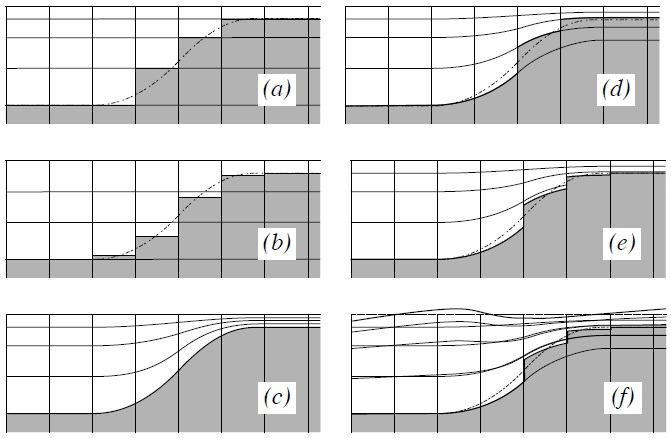
\includegraphics[width=\linewidth]{NEMOP58.jpg}
  \caption{An illustration of different veritcal coordinate systems available in NEMO. \citep{Madec2011}. (a) z-coordinate, (b) z-coordinate with partial cells, (c) s-coordinate, (d) hybrid s-z coordinate, (e) hybrid s-z coordinate with partial cell, (f) shows (e) with a non-linear free surface (which can be used with any coordinate system).}
  \label{FIG:coords}
\end{figure}

The main difficulty in comparing different vertical coordinate systems lies in the availability of a 'control' case for the comparison. With the wide selection of models available to researchers, it is not only the vertical coordinate system which differs but also the numerical schemes being used to resolve various processes. This could lead to false similarities or differences and cause incorrect conclusions. \citep{Ezer2016b} was able to compare results from z-coordinate models and s-coordinate models while minimalising any other differnces between the models. Although the z-coordinate models are capable of producing an accurate Gulf Stream at hight resolutions, the s-coordinate models provided a more accurate representation when restricted with coarser models. However, as \citep{Ezer2016b} noted in the comparison, partial and shaved cells (whereby corners of the cells are 'shaved' off to smooth out slopes) were not used in any of these models.



\end{document}
